%\chapter{Background}  \label{background}
\chapter{Background}  \label{background}

\NZ{I noticed all "anti-unification" words are modified to "antiunification", is that a change that you have made? I just want to double check it with you to make sure that it is right.}
\RW{Yes, I did that.  They are equivalent.  This allowed me to make some other global corrections.}

A programming language is described by the combination of its syntax and semantics. The syntax concerns the legal structures of programs written in the programming language, while the semantics is about the meaning of every construct in that language. Furthermore, the abstract syntactic structure of source code written in a programming language can be represented as an \emph{abstract syntax tree} (AST), in which nodes are occurrences of syntactic structures and edges represent nesting relationships. In order to construct structural generalizations describing the commonalities and differences between logged Java methods (LJMs), it is important to first understand what AST is and how specific information about each Java element is held in an AST\@. An investigation of the application of antiunification and its extensions on this structure to produce structural generalizations is also needed. In addition, it is necessary to figure out how the Jigsaw framework could be used to determine potential candidate structural correspondences.
\RW{This paragraph could use a bit of expansion.  I would phrase it more in terms of why you will be telling the reader about these things.  This chapter explains some key ideas and background research that are necessary to understand the extensions being made in this thesis.  I changed my mind about the order: the theory of antiunification does not need ASTs.  I would explain that a term can be represented as a tree or vice versa.}

In this chapter, antiunification is summarized in section~\ref{AU}, starting with an introduction to unification and its dual antiunification, followed by a discussion regarding to limitations of antiunification to address our problem.
Sections~\ref{AST} and~\ref{AUAST} will provide a brief description of the AST structure and its extended form, both are necessary to understand the requirements that guide the development of an antiunification algorithm for our application.
Section~\ref{HOAUMT} is dedicated to explaining higher-order antiunification modulo theories (HOAUMT), which is an extension to antiunification, where a set of equivalence theories are defined and applied on higher-order extended structures to incorporate background knowledge.
Lastly, this chapter will discuss the Jigsaw framework and its application in determining potential candidate structural correspondences in Section~\ref{Jigsaw}.

\section{Antiunification}   \label{AU}

This section will introduce a formal definition of a term, the application of a substitution on a term, and the definition of an instance and an anti-instance of a term, as the requirements needed  to describe unification theory and its dual antiunification theory.
%to understand the theories in order

\begin{defn}[Term]\label{def:term}
A term is defined to be a variable, a constant, or a function symbol followed by a list of terms as the arguments of the function.
\end{defn}

Function symbols taking n arguments are called n-ary function symbols, and 0-ary function symbols are called constants. The identifiers starting with a lowercase letter are used to represent function symbols (e.g., $f(a,b)$, $g(a,b)$) and constants (e.g., $a$, $b$), while variables are represented by identifiers starting with an uppercase letter (e.g., $X$, $Y$). The followings are examples of a term:
\begin{itemize} [leftmargin=0.7in]
\item $Y$
\item $a$
\item $f(X, c)$
\item $f(g(X, b),Y, g(a, Z))$
\end{itemize}
%A term is called grounded if it does not contain any variables (e.g., $f(a,b)}), and
\begin{defn}[Substitution]\label{def:substitution}
A substitution is a set of pairs of variables and terms, each denotes a mapping from a variable to a term.
\end{defn}

\begin{defn}[Applying a substitution]\label{def:substitution}
Applying a substitution to a term results in the replacement of all occurrences of each variable of the term defined in the substitution set by its corresponding term.
\end{defn}

As an example, an application of a substitution $\Theta$ = ({$X \rightarrow a, Y \rightarrow b $})
on a term $f(X,Y)$ results in the replacement of all occurrences of the variable $X$ by the term $a$ and all occurrences of the variable $Y$ by the term $b$, and thus $f(X,Y)\xrightarrow{\Theta} f(a,b)$.



\begin{defn}[Instance \& anti-instance]\label{def:instance}
$a$ is an instance of a term $X$ and $X$ is an anti-instance of $a$, if there is a substitution $\Theta$ such that the application of $\Theta$ on $X$ results in $a$ ($X\xrightarrow{\Theta}a$).
\end{defn}

\begin{defn}[Unifier]\label{def:unifier}
A unifier is a common instance of two given terms.
\end{defn}

Unification usually aims to create the \emph{most general unifier} (MGU), that is, $U$ is the MGU of two terms such that for all unifiers $U'$ there exists a substitution $\Theta$ such that $U\xrightarrow{\Theta}U'$. Unification aims to make a more concrete structure in essence, whereas what we need is a more generalized structure, which leads to the use of the dual of unification.

\begin{defn}[Generalization]\label{def:generalization}
$X$ is a generalization for $a$ and $b$, where $X$ is an anti-instance for $a$ and $b$ under substitutions $\Theta_1$ and $\Theta_2$, respectively ($X\xrightarrow{\Theta_1}a$ and$X\xrightarrow{\Theta_2}b$).
\end{defn}
To create a generalization of two given terms, the inverse of unification should be used, which is called \emph{antiunification}, where the two original terms are the instances of the new antiunified term.

\begin{defn}[Antiunifier]\label{def:antiunifier}
An antiunifier is a common generalization of two given terms.
\end{defn}

An antiunifier contains common pieces of the original terms, while the differences are abstracted away using variables. An antiunifier for a pair of terms always exists since we can antiunify any two terms by creating a variable $X$. However, antiunification usually aims to find the \emph{most specific antiunifier} (MSA), that is , $A$ is the MSA of two structures where there exists no antiunifier $A'$ such that $A\xrightarrow{\Theta}A'$.

As an example, the antiunifier of two given terms $f(X,b)$ and $f(a,Y)$ is the new term $f(X,Y)$, containing common pieces of the two original terms. The variable $Y$ in the antiunifier $f(X,Y)$ can be substituted by the term $b$ to re-create $f(X,b)$ (with $\Theta_1 = Y\xrightarrow{}b$) and the variable $X$ in the antiunifier can be substituted by the term $a$ to re-create $f(a,Y)$
(with $\Theta_2 = X\xrightarrow{\Theta}a$), as depicted in Figure~\ref{fig:uni-anti-uni}.
In addition, the unifier $f(a,b)$ of the two terms can be instantiated by applying the substitutions $\Theta_1'=X\xrightarrow{\Theta}a$ and $\Theta_2'=Y\xrightarrow{\Theta}b$ on the terms $f(X,b)$ and $f(a,Y)$, respectively.

\begin{figure} [H]
  \[
\begin{tikzcd}[column sep=small]
&
  {\makecell[l]{\hspace{0.4cm}f(X,Y)\\\text{antiunifier}}}
  \arrow{dr}{\Theta_2 = X \rightarrow a}
  \arrow[->,swap]{dl}{\Theta_1 = Y \rightarrow b} % <-- reflect the direction of the hook
\\
f(X,b)
 \arrow[->,swap]{dr}{\Theta_1' = X \rightarrow a}
 %\arrow{dr}
&&
f(a, Y)
  \arrow{dl}{\Theta_2' = Y \rightarrow b}
  \\
&
{\makecell[l]{f(a,b)\\\text{unifier}}}
\end{tikzcd}
\]
  \caption{The unification and antiunification of the terms $f(X,b)$ and $f(a,Y)$.}
  \label{fig:uni-anti-uni}
\end{figure}

MSA should preserve as much of common pieces of both original terms as possible; however, antiunification fails to capture complex commonalities as it restricts substitutions to only replace first-order variables by terms. That is, when two terms differ in function symbols, antiunification fails to capture common details of them. For example, the antiunifier of the terms $f(a,b)$ and $g(a,b)$ is $X$ using antiunification as depicted in Figure~\ref{fig:first-anti-uni}.
% replace ot to be replaced?

\begin{figure} [H]
\[
\begin{tikzcd}[column sep=small]
&
  X
  \arrow{dr}{\Theta_2 = X \rightarrow g(a,b)}
  \arrow[->,swap]{dl}{\Theta_1 = X \rightarrow f(a,b)} % <-- reflect the direction of the hook
\\
f(a,b)
&&
g(a,b)
\end{tikzcd}
\]
  \caption{The antiunification of the terms $f(X,b)$ and $f(a,Y)$.}
  \label{fig:first-anti-uni}
\end{figure}

An extended form of antiunification, which is called higher-order antiunification, would allow us to create MSA by extending the set of possible substitutions such that variables can be replaced by not only constants but also functional symbols to retain the detailed commonalities. For example, the antiunifier of the terms $f(a,b)$ and $g(a,b)$ is $X(a,b)$ using higher-order antiunification as depicted in Figure~\ref{fig:higher-anti-uni}.
\begin{figure} [H]
\[
\begin{tikzcd}[column sep=small]
&
  X(a,b)
  \arrow{dr}{\Theta_2 = X \rightarrow g}
  \arrow[->,swap]{dl}{\Theta_1 = X \rightarrow f} % <-- reflect the direction of the hook
\\
f(a,b)
&&
g(a,b)
\end{tikzcd}
\]
  \caption{The higher-order antiunification of the terms $f(X,b)$ and $f(a,Y)$.}
  \label{fig:higher-anti-uni}
\end{figure}

In the following sections, a brief description of the AST structure and the application of antiunification on its extended form to construct structural generalizations will be provided.

\section{Abstract Syntax Tree}   \label{AST}
% JDT
\RW{Explain what an AST is before talking about details of the JDT.  Show us tree-based representations of code.  Then show us JDT-based representations.}

The Eclipse Java Development Tools (JDT) framework provides APIs to access and manipulate Java source code via Abstract Syntax Tree (AST). AST maps Java source code in a tree structure form and thus every Java source code can be represented as tree of AST nodes, where each represents an element of the Java Programming Language. AST helps developers to modify and analyze the Java program in a more convenient way than text-bases source code by providing a language parser of the Java source code, determining the bindings between name and type references, and providing specific information of each Java element. For example, the simple AST structure of two sample logged Java classes in Figures~\ref{ch3-ex1} an~\ref{ch3-ex2} is shown in Figure~\ref{fig:ast}

%We introduce an example to illustrate the antiunification process over two ASTs, and so

\begin{figure}[H]
\def\baselinestretch{1}
\begin{lstlisting}
public abstract class EBPlugin extends EditPlugin implements EBComponent {
    private Boolean seenWarning;
  
    protected EBPlugin() {
    }

    public void handleMessage(EBMessage message) {
        if(seenWarning) return;
        seenWarning = true;
        Log.log(Log.WARNING, this, getClassName() + " should extend EditPlugin not EBPlugin since it has an empty" + handleMessage());
    }
}
\end{lstlisting}
\caption{A Java class that uses a logging call. This will be referred to as Example 1.\label{ch3-ex1}}
\end{figure}


\begin{figure}[H]
\def\baselinestretch{1}
\begin{lstlisting}
public static class Wrapper implements ActionListener {
    private ActionContext context;
    private String actionName;

    public Wrapper(ActionContext context,  String actionName) {
        this.context = context;
        this.actionName = actionName;
    }
    
    public void actionPerformed(ActionEvent evt) {
        EditAction action = context.getAction(actionName);
        if(action == null) {
            Log.log(Log.ERROR, this, "Unknown action: " + actionName);
        }
        else
            context.invokeAction(evt, action);
    }
}
\end{lstlisting}
\caption{A Java class that uses a logging call. This will be referred to as Example 2.\label{ch3-ex2}}
\end{figure}

\begin{figure} [p]
  \centering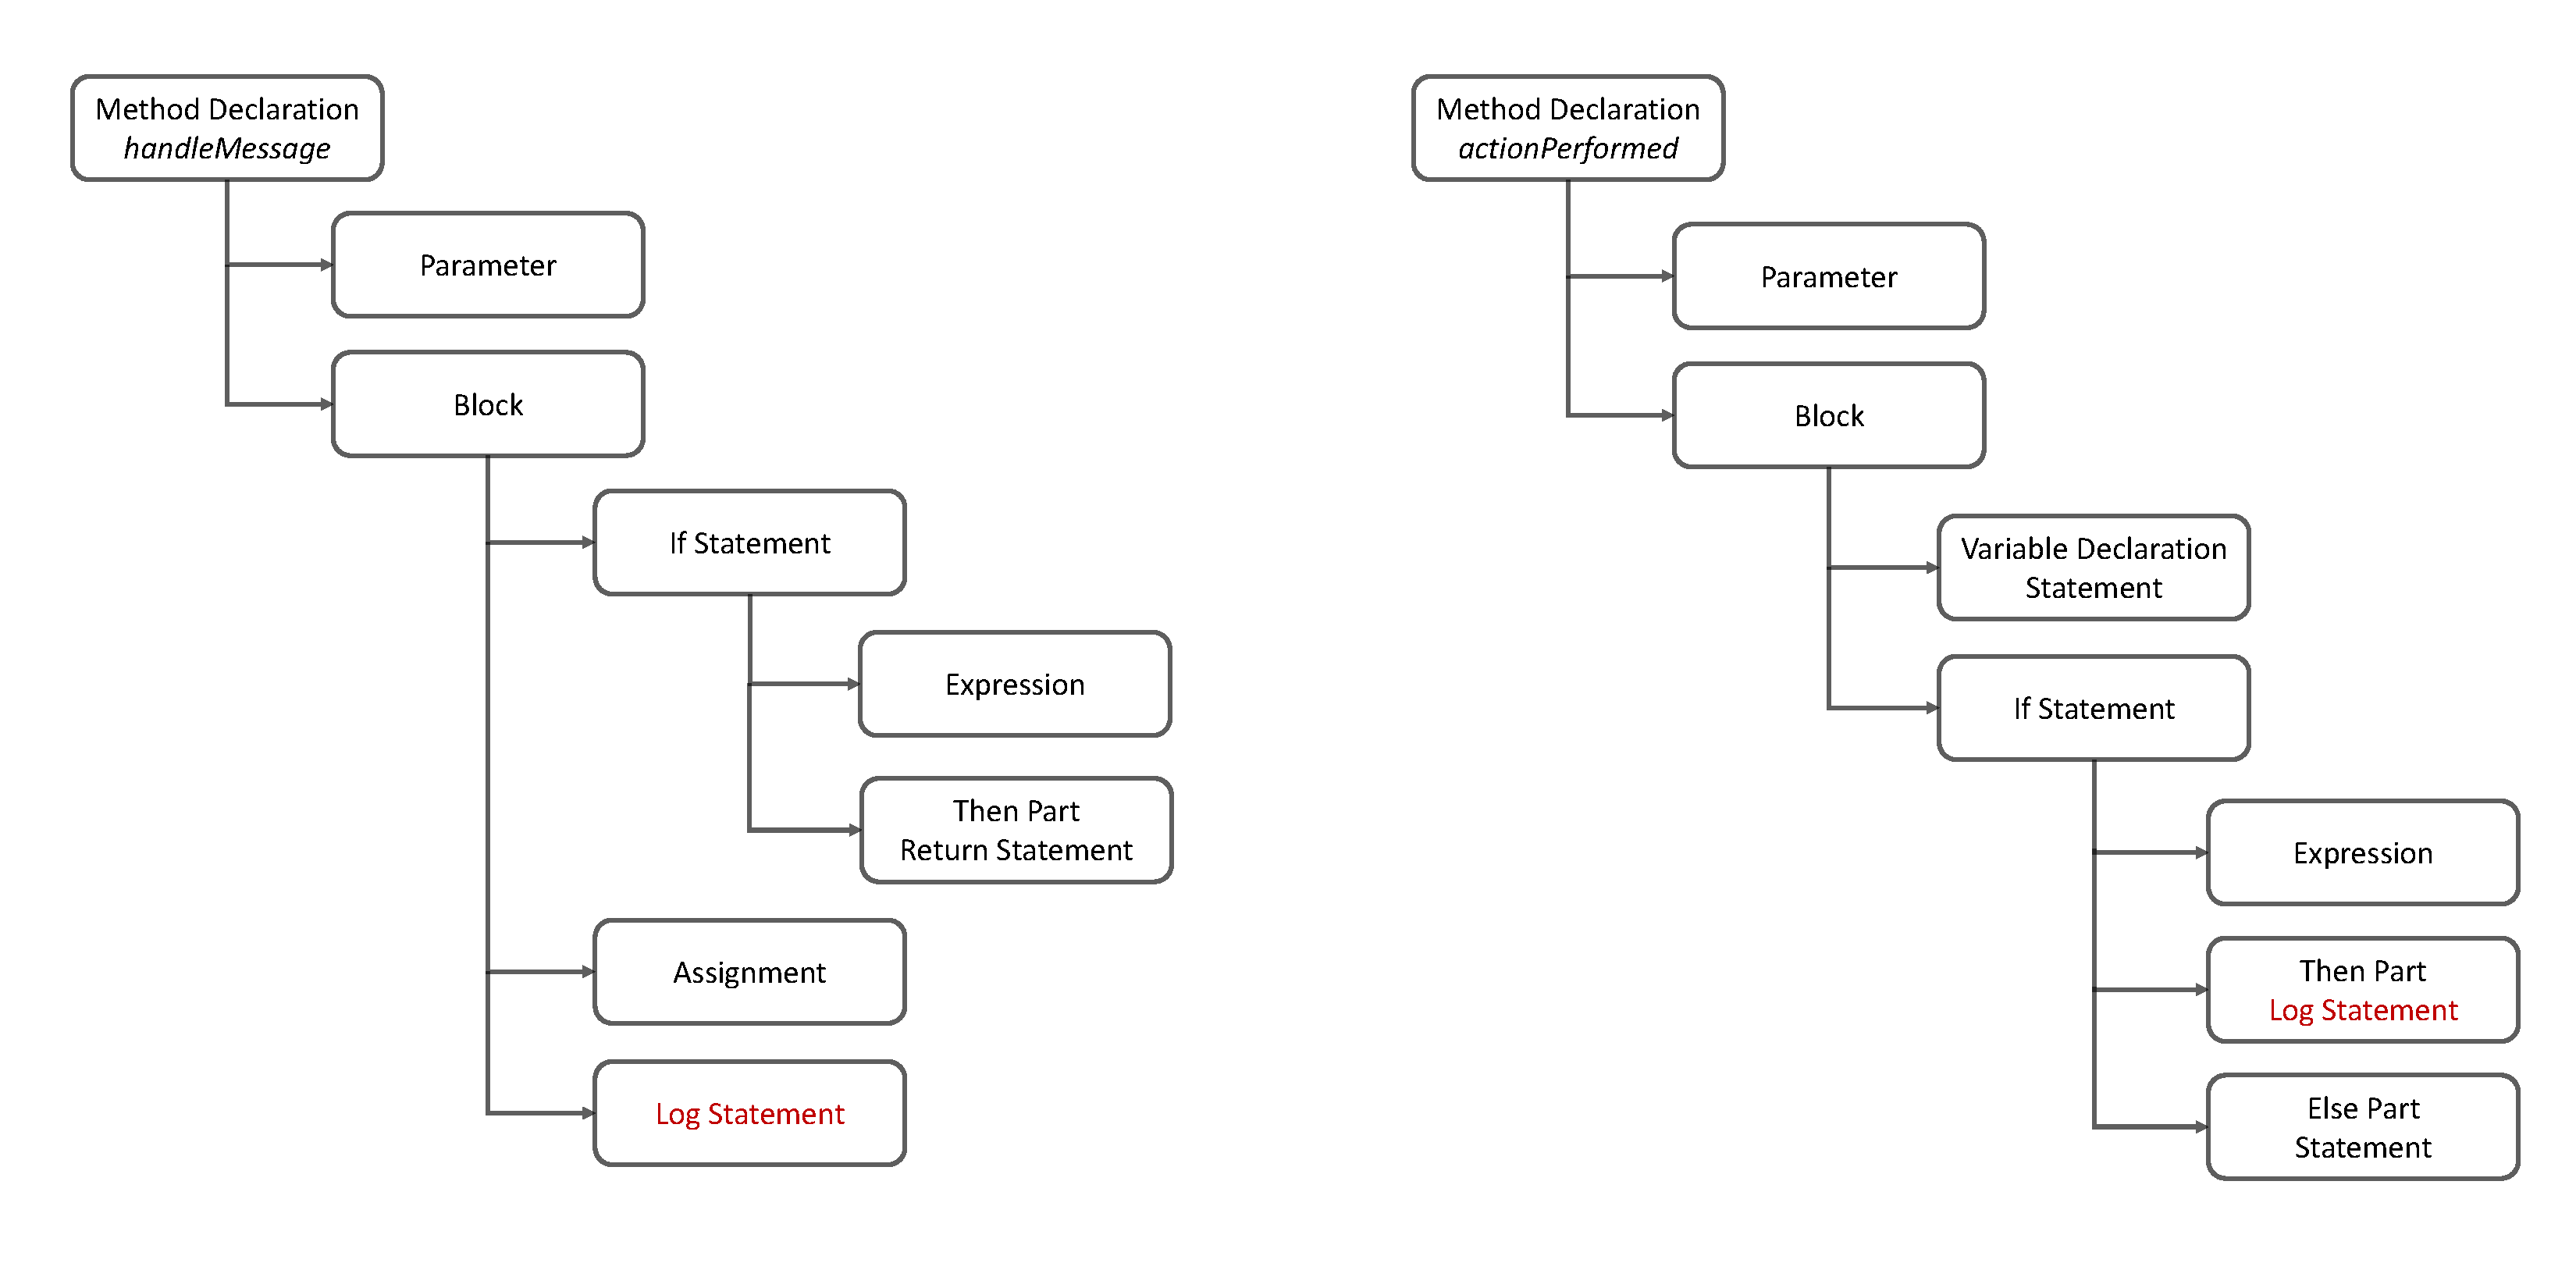
\includegraphics[width = \textwidth]{Drawing4/AST.pdf}
  \caption{Simple AST structure of examples in Figures~\ref{ch3-ex1} and~\ref{ch3-ex2}.}
  \label{fig:ast}
\end{figure}

In the JDT framework, structural properties of each AST node can be used to obtain specific information of the Java element that it represents. These properties are stored in a map data structure that associates each property to its value and are divided into three types:
\begin{itemize} [leftmargin=0.7in]
\item \textit{Simple structural properties:} that contain a simple value which has a primitive or simple type or a basic AST constant (e.g., identifier property of a name node whose value is a String)
\item \textit{Child structural properties:} where the value is a single AST node (e.g., name property of a method declaration node)
\item \textit{Child list structural properties}: where the value is a list of child nodes (e.g., body declarations property of a class declaration node whose value is a list of body declaration nodes, including method declaration and field declaration nodes.)
\end{itemize}
%AST is made up of AST nodes as subtrees and simple values as leaves.
An instance of an AST structure can be represented in an abstract form that can be mapped to the definition of a term described in Section~\ref{AU}. As an example, the ASTs of the logging calls at line~10 of Figure~\ref{ch3-ex1} and line~13 of Figure~\ref{ch3-ex2} can be represented respectively as:
%\RW{These ASTs were messed up.  I fixed them according to what the code says, picking some meaningful names for the AST nodes.}
\begin{itemize} [leftmargin=0.7in]
%\item expr(expr(\code{Log}), name(\code{log}), args(leftop(\code{message}), +, \\rightop(\code{" is empty"}), qual(\code{Log}), name(\code{WARNING})))
%\item \textit{expression(expression(Log), name(log), arguments(leftoperand(actionName),\\+, rightoperand("is an unknown action"), qualifier(Log), name(WARNING)))}
\item \textit{methodCall}(\\
\hspace*{1em}\textit{qualifiedName}(\code{Log}, \textit{simpleName}(\code{log})),\\
\hspace*{1em}\textit{arguments}(\\
\hspace*{2em}\textit{qualifiedName}(\code{Log}, \mbox{\textit{simpleName}(\code{WARNING})}),\\
\hspace*{2em}\textit{thisExpression}(),\\
\hspace*{2em}\textit{additionExpression}(\\
\hspace*{3em}\textit{methodCall}(\textit{simpleName}(\code{getClassName}), \textit{arguments}()),\\
\hspace*{3em}\textit{stringLiteral}(..),\\
\hspace*{3em}\textit{methodCall}(\textit{simpleName}(\code{handleMessage}), \textit{arguments}())\\
\hspace*{2em})\\
\hspace*{1em})\\
)
\item \textit{methodCall}(\\
\hspace*{1em}\textit{qualifiedName}(\code{Log}, \textit{simpleName}(\code{log})),\\
\hspace*{1em}\textit{arguments}(\\
\hspace*{2em}\textit{qualifiedName}(\code{Log}, \mbox{\textit{simpleName}(\code{ERROR})}),\\
\hspace*{2em}\textit{thisExpression}(),\\
\hspace*{2em}\textit{concatenationExpression}(\\
\hspace*{3em}\textit{stringLiteral}(..),\\
\hspace*{3em}\textit{simpleName}(\code{actionName})\\
\hspace*{2em})\\
\hspace*{1em})\\
)
%\item methodCall(qualifiedName(\code{Log}, simpleName(\code{log})), args(qualifiedName(Log, simpleName(ERROR)), thisExpr(), concatExpr(stringLiteral(..), simpleName(\code{actionName}))))
\end{itemize}
(Details of the specific string literals are elided for this presentation.)

Here, the non-leaf AST nodes (e.g., \textit{methodCall}, \textit{simpleName}, \textit{thisExpression}) can be viewed as function symbols while leaf nodes (e.g., \code{log}, \code{WARNING}) can be viewed as constants in the term definition. As described in Section~\ref{AU}, antiunification utilizes variables that must be substituted with proper structures to re-create original structures. However, the AST structure does not contain any variables and so we need to construct an extended form of AST, which will be described in the following section.

% In order to map an instance of an AST to that form of structure, first we should understand how an AST structure holds its subtrees and leaves
%The goal of this phase is to construct an extension of the AST structure that would allow the creation of an antiunified structure.

\section{Constructing the AUAST} \label{AUAST}
An antiunifier AST (AUAST) is an extended form of AST that allows the insertion of variables in place of any node in the tree structure, including both subtrees and leaves, to indicate variations between original structures. The AUAST addresses the limitations of AST to construct an antiunifier by adding the following structural properties:
\begin{itemize} [leftmargin=.4in]
\item \textit{Simple Variable Property}: an extension of simple property referring to two simple values to allow the insertion of variables in place of leaves.
\end{itemize}
\begin{itemize} [leftmargin=.4in]
\item \textit{Child Variable Property}: an extension of child property referring to two child AST nodes to allow the insertion of variables in place of subtrees.
\end{itemize}
The antiunification of AUASTs of logging calls in Figures~\ref{ch3-ex1} and~\ref{ch3-ex2} is depicted in Figure~\ref{fig:logging-anti}. The new variables $X$ and $Y$ are created to abstract away the structural variations.
%\item it can be mapped to our recursive definition of a term, where AST nodes and simple values may be viewed as function-symbols and constants, respectively


\begin{figure} [H]
\begin{small}
\[
\begin{tikzcd}[column sep=small]
&\makebox[1in][c]{\makecell[l]{%
\text{\textit{methodCall}(}\\
\text{\hspace*{1em}\textit{qualifiedName}(\textsf{\footnotesize Log}, \textit{simpleName}(\textsf{\footnotesize log})),}\\
\text{\hspace*{1em}\textit{arguments}(}\\
\text{\hspace*{2em}\textit{qualifiedName}(\textsf{\footnotesize Log}, \mbox{\textit{simpleName}(\textit{X})}),}\\
\text{\hspace*{2em}\textit{thisExpression}(),}\\
\text{\hspace*{2em}\textit{Y}))}\\*[3em]
%\text{\hspace*{1em})}\\
%\text{)}\\
}}
\arrow{dr}{\Theta_2 = (X \rightarrow \text{ \code[basicstyle=\scriptsize\sffamily]{ERROR}}, Y \rightarrow \text{ \textit{additionExpression}(..)})}
\arrow[->,swap]{dl}{\Theta_1 = (X \rightarrow \text{ \code[basicstyle=\scriptsize\sffamily]{WARNING}}, Y \rightarrow \text{ \textit{concatenationExpression}(..)})} % <-- reflect the direction of the hook
\\
\makebox[2in][l]{\makecell[l]{\vspace*{1em}\\%
\text{\textit{methodCall}(}\\
\text{\hspace*{1em}\textit{qualifiedName}(\textsf{\footnotesize Log}, \textit{simpleName}(\textsf{\footnotesize log})),}\\
\text{\hspace*{1em}\textit{arguments}(}\\
\text{\hspace*{2em}\textit{qualifiedName}(\textsf{\footnotesize Log},}\\ \text{\hspace*{3em}\mbox{\textit{simpleName}(\textsf{\footnotesize WARNING})}),}\\
\text{\hspace*{2em}\textit{thisExpression}(),}\\
\text{\hspace*{2em}\textit{additionExpression}(..)))}\\
}\hspace*{1em}}&&
\makebox[2in][l]{\makecell[l]{\vspace*{1em}\\%
\text{\textit{methodCall}(}\\
\text{\hspace*{1em}\textit{qualifiedName}(\textsf{\footnotesize Log}, \textit{simpleName}(\textsf{\footnotesize log})),}\\
\text{\hspace*{1em}\textit{arguments}(}\\
\text{\hspace*{2em}\textit{qualifiedName}(\textsf{\footnotesize Log},}\\ \text{\hspace*{3em}\mbox{\textit{simpleName}(\textsf{\footnotesize ERROR})}),}\\
\text{\hspace*{2em}\textit{thisExpression}(),}\\
\text{\hspace*{2em}\textit{concatenationExpression}(..)))}\\
}}
\end{tikzcd}
\]
\end{small}
\caption{The antiunification of AUASTs of logging calls in Examples 1 and 2.\label{fig:logging-anti}}
\end{figure}
%The AUASTs of log Method Invocation nodes from the Java classes in Figure~\ref{ch3-ex1} and Figure~\ref{ch3-ex2}.

Applying higher-order antiunification on AUAST structures could help to construct a structural generalization by maintaining the common pieces and abstracting the differences away using variables. However, it is not comprehensive enough to solve our problem as it does not consider background knowledge about AST structures, such as syntactically different but semantically relevant structures, missing structures, and different ordering of arguments. In the following section, we will look at an extension of antiunification, higher-order antiunification modulo theories, and how it can sufficiently address the limitations of antiunification in our context.


\section{Higher-order antiunification modulo theories}   \label{HOAUMT}
%antiunification cannot incorporate any background knowledge such as sematic knowledge required to solve our problem, and we should apply an extended form of antiunification, called higher-order antiunification modulo theories, where a set of equivalence equations is defined to incorporate semantic knowledge of structural equivalences supported by the Java language specification. An equivalence equation $=_E$ determines which terms are considered equal, and the set of equivalence equations must be applied on higher-order extended structures to allow the antiunification of AST structures that are not identical but are semantically equivalent.
In higher-order antiunification modulo theories, a set of equivalence equations is defined to incorporate background knowledge. Each equivalence equation $=_E$ determines which terms are considered equal and a set of these equations can be applied on higher-order extended structures to determine structural equivalences. For example, we have introduced an equivalence equation $=_E$, such that $f(X,Y) =_E f(Y,X)$ to indicate that the ordering of arguments does not matter in our context.

% nil restriction!!!!
We have also introduced a theory, called NIL-theory, that adds the concept of NIL structure, which is defined to create a structure out of nothing, and defines an equivalence equation $=_E$ for it. The NIL structure can be used to antiunify two structures when a substructure exists in one but is missing from the other. However, some requirements should be taken to avoid the overuse of NIL structures such that the original structures must have common substructures but vary in the size for dissimilar substructures. For example, we can antiunify the two structures $b$ and $f(a,b)$ through the application of NIL-theory by creating the term $nil(nil,b)$ which is $=_E$ to $f(b)$ and antiunifying $nil(nil,b)$ with $f(a,b)$ as depicted in Figure~\ref{fig:anti-nil}.
% to introduce an equivalence equation =E for the NIL structure
% it should be modified
% should it be different?
\begin{figure} [H]
\[
\begin{tikzcd}[column sep=small]
&
  X(Y,b)
  \arrow{dr}{\Theta_2 = ( X \rightarrow nil, Y \rightarrow nil) }
  \arrow[->,swap]{dl}{\Theta_1 = ( X \rightarrow f, Y \rightarrow a)} % <-- reflect the direction of the hook
\\
f(a,b)
&&
nil(nil,b) =_E  b
\end{tikzcd}
\]
  \caption{ The antiunification of the terms f(a, b) and nil(nil,b).}
  \label{fig:anti-nil}
\end{figure}


We have also defined a set of equivalence equations to incorporate semantic knowledge of structural equivalences supported by the Java language specification as it provides various ways to define the same language specifications. These theories should be applies on higher-order extended structures to antiunify AST structures that are not identical but are semantically equivalent. For example, consider for- and while- statements that are two types of looping structure in Java programming language that have different syntax but semantically cover the same concept. Let us look at the \code{for(i=0;i<10;i++)} and \code{while(i<10)} code snippets, whose AST structures can be represented as \code{for(initializer(i,=,0),expression(i,<,10), updaters(i,++))} and \code{while(expression(i,<,10))}, respectively. We could define an equivalence equation $=_E$ that allows the antiunification of for- and while- statements which are semantically similar structures. We also need to utilize the NIL-theory to handle varying number of arguments as the for- loop has three arguments whereas the while- loop only has one. Using the NIL-theory we can create the structure \code{while(nil(nil,nil,nil),expression(i,<,10), nil(nil,nil))} that is $=_E$ to \code{while(expression(i,<,10))} and construct the antiunifier, \code{V_0(V_1(V_2,V_3,V_4),expression(i,<,10), V_5(V_2,V_6))} as depicted in Figure~\ref{fig:for-while}.

\begin{figure} [H]
\[
\begin{tikzcd}[column sep=small]
&
  \makecell[l]{V_0(V_1(V_2,V_3,V_4),\\expression(i,<,10),\\ V_5(V_2,V_6)) }
  \arrow{dr}{\Theta_2 = \makecell[l]{ V_0 \rightarrow while, V_1 \rightarrow nil,\\ V_2 \rightarrow nil, V_3 \rightarrow nil,\\ V_4 \rightarrow nil, V_5 \rightarrow nil, V_6 \rightarrow nil} }
  \arrow[->,swap]{dl}{\Theta_1 = \makecell[l]{V_0 \rightarrow for, V_1 \rightarrow initializer, \\V_2 \rightarrow i, V_3 \rightarrow =, V_4 \rightarrow 0, \\V_5 \rightarrow updaters, V_6 \rightarrow ++ }} % <-- reflect the direction of the hook
\\
  \makecell[l]{for(initializer(i,=,0),\\expression(i,<,10),\\ updaters(i,++))}
&&
  \makecell[l]{while(nil(nil,nil,nil),\\expression(i,<,10),\\ nil(nil,nil)) }
\end{tikzcd}
\]
  \  \caption{ The antiunification of the structures \code{for(initializer(i,=,0),expression(i,<,10), updater(i,++))} and \code{while(nil(nil,nil,nil),expression(i,<,10), nil(nil,nil))}.}
  \label{fig:for-while}
\end{figure}
% higher-order extension and the equational theories
% provide a better example
However, defining complex substitutions in higher-order antiunification modulo theories results in losing the uniqueness of MSA. For example, consider the terms $f(g(a,e))$ and $f(g(a,b),g(d,e))$. As described in Figure~\ref{fig:multipleMSA}, two MSAs exist for these terms: we can antiunify $g(a,e)$ and $g(a,b)$ to create the antiunifier $g(a,X_0)$ and antiunify $g(d,e)$ with the NIL structure to create the antiunifier $Y(Z,X_1)$; or we can antiunify $g(a,e)$ and $g(d,e)$ to create the antiunifier $g(X_0,e)$ and antiunify $g(a,b)$ with the NIL structure to create the antiunifier $Y(Z,X_1)$.

\begin{figure} [H]
\[
\begin{tikzcd}[column sep=small]
&
  f(g(X_0,e),Y(Z,X_1))
  \arrow{dr}{\Theta_2 = ( X_0 \rightarrow a, Y \rightarrow nil, Z \rightarrow nil, X_1 \rightarrow nil) }
  \arrow[->,swap]{dl}{\Theta_1 = ( X_0 \rightarrow d, Y \rightarrow g, Z \rightarrow a, X_1 \rightarrow b)} % <-- reflect the direction of the hook
\\
f(g(a,b), g(d,e))
&&
f(g(a,e))
\end{tikzcd}
\]	

\[
\begin{tikzcd}[column sep=small]
&
  f(g(a,X_0),Y(Z,X_1))
  \arrow{dr}{\Theta_2 = ( X_0 \rightarrow e, Y \rightarrow nil, Z \rightarrow nil, X_1 \rightarrow nil) }
  \arrow[->,swap]{dl}{\Theta_1 = ( X_0 \rightarrow b, Y \rightarrow g, Z \rightarrow d, X_1 \rightarrow e)} % <-- reflect the direction of the hook
\\
f(g(a,b), g(d,e))
&&
f(g(a,e))
\end{tikzcd}
\]
  \caption{The antiunification of the terms $f(g(a,b), g(d,e))$
and $f(g(a,e))$ that creates multiple MSAs.}
  \label{fig:multipleMSA}
\end{figure}


Despite having multiple potential MSAs, we need to determine one single MSA that is the most appropriate in our context. However, the complexity of finding an optimal MSA is undecidable in general [Cottrell et al., 2008] since an infinite number of possible substitutions can be applied to every variable. Therefore, we need to use an approximation technique to construct one of the best MSAs that can sufficiently solve our problem.
% reason since?
%Our goal is to find an MSA that is an approximation of the best fit to our application


\section{The Jigsaw framework}  \label{Jigsaw}
The Jigsaw tool is developed by \citet{cottrell2008semi} to determine the structural correspondences between two Java source code fragments through the application of higher-order antiunification modulo theories such that one fragment can be integrated to the other one for small scale code reuse. Jigsaw could help determine potential candidate structural correspondences between AST nodes of logged Java classes by producing an augmented form of AST, called CAST (Correspondence AST), where each node holds a list of candidate correspondence connections between the two structures, each representing an antiunifier. It also develops a measure of similarity to indicate how similar the nodes involved in each correspondence connection are. The Jigsaw similarity function relies on structural correspondence along with a simple knowledge of semantic equivalences supported by the Java language specification. It returns a value between 0 and 1 that indicates zero and total structural matching, respectively. In addition, several semantical heuristics are used to improve the accuracy of similarity measurement by allowing the comparison of AST nodes that are not syntactically identical but are semantically related to each other.

For example, the similarity between names of AST nodes is measured using a normalized computation based on the length of longest common substring. The comparison of \code{int} and \code{long} variable types is another example, where an arbitrary value of 0.5 is defined as the similarity value as they are not syntactically identical but are not semantically unrelated. In addition, the Jigsaw framework also detects the structural correspondence between  for-, enhanced-for-, while-, and do- loop statements; and if- and switch- conditional statements. As an example, Figure~\ref{fig:meth-ast-1} shows the structural correspondence connections created by Jigsaw between the AST nodes of Examples 1 and 2 along with the similarity value for each correspondence connection.

\begin{figure} [H]
  \centering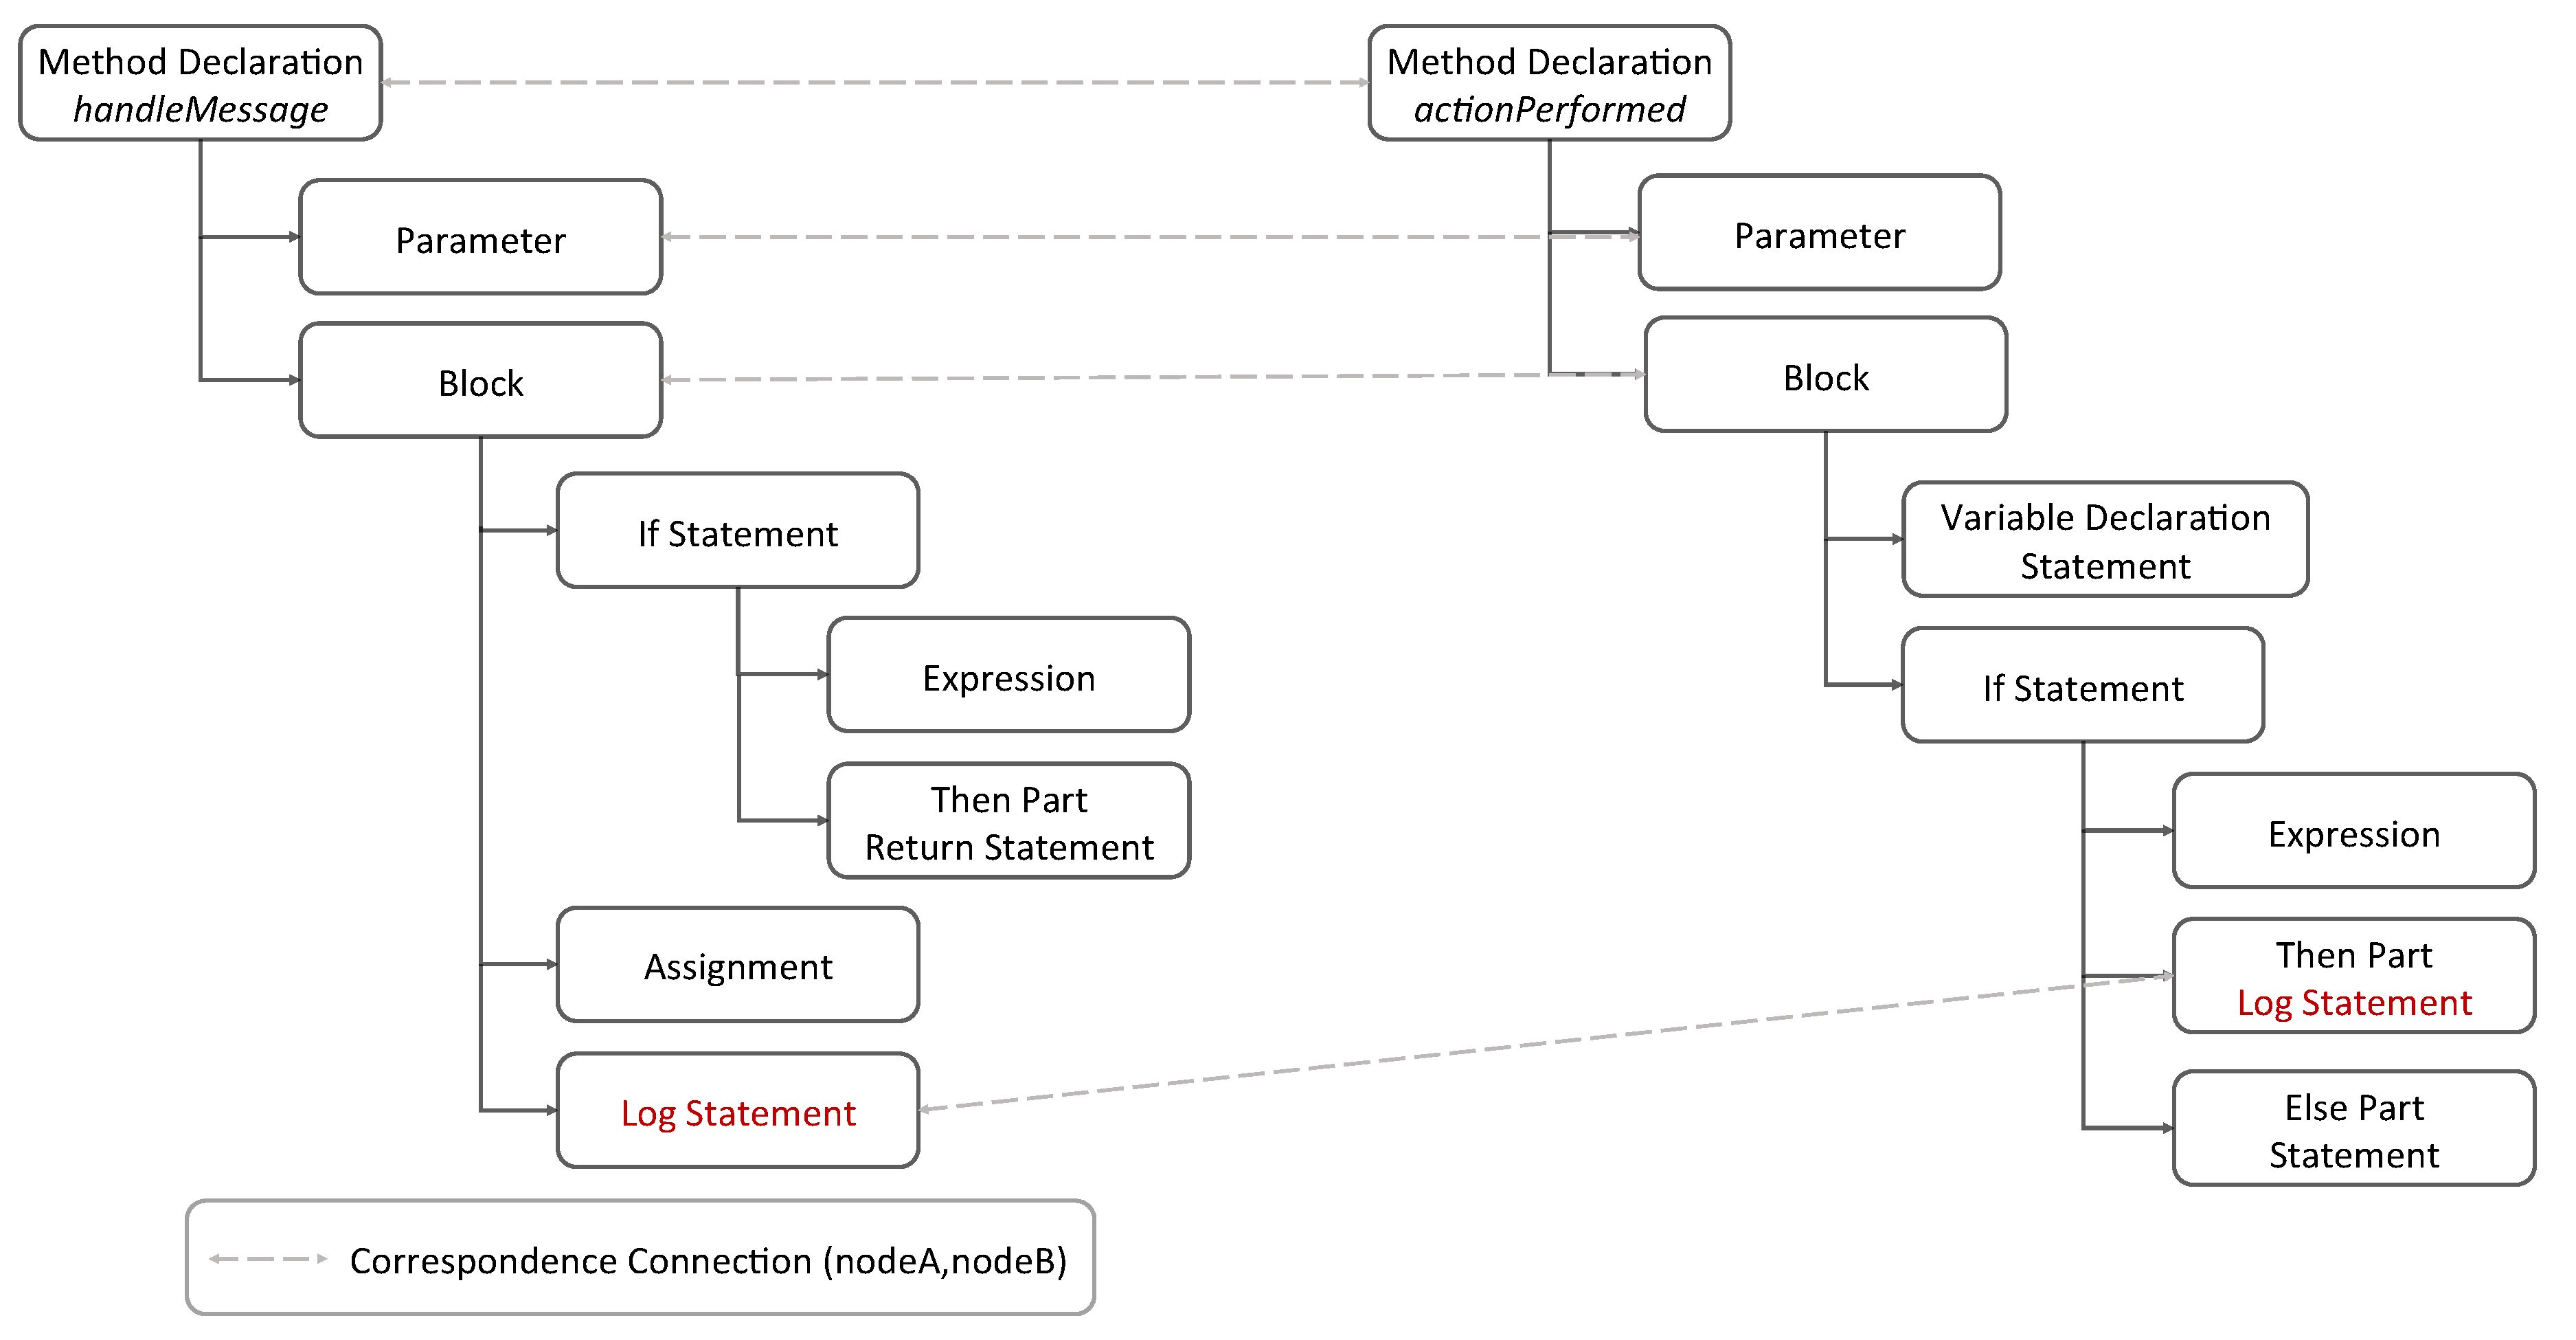
\includegraphics [width = \textwidth]{Drawing4/FirstCorr.pdf}
  \caption{Simple CAST structure of examples in Figures~\ref{ch3-ex1} and~\ref{ch3-ex2}. The links between AST nodes indicate structural correspondence connections created by the Jigsaw framework along with the similarity value.}
  \label{fig:meth-ast-1}
\end{figure}

However, the Jigsaw tool does not suffice to construct an antiunifier that is the best fit to our application. In addition, the Jigsaw similarity function does not measure the similarity of two logged Java classes with a focus on logging calls, which is needed in our context. To address these issues, we should develop a greedy selection algorithm to approximate the best antiunifier by determining the best correspondence for each node. In the following chapter, we will discuss our approach to construct structural generalizations and our implementation by means of the higher-order antiunification modulo theories and the Jigsaw framework.

 
\section{Summary}  \label{summary}
In this chapter, we described antiunification as a technique to construct a common generalization of two given terms. We have also introduced an extended form of antiunification, which is called higher-order antiunification modulo theories, where a set of equivalence equations can be applied on higher-order extended structures to incorporate background knowledge. In addition,
we provided a brief description of AST that maps Java source code in a tree structure form, and why an extended form of it, named AUAST, is required to create higher-order structures specific to our problem context. Finally, we discuss the Jigsaw framework and how it could assist us in determining the potential structural correspondences.
